\documentclass{article}
\usepackage{array}
\usepackage{graphicx} % Required for inserting images

\title{Implementacija histograma in vzporednega scan algoritma}
\author{Tim Rekelj, 63210277}
\date{February 2024}

\begin{document}

\maketitle

\newpage
\section{Kazalo}
\renewcommand*\contentsname{}
\tableofcontents

\newpage
\section{Uvod}
Izenačevanje slike je postopek, ki se uporablja za izboljšanje kontrasta slike in poudarjanje podrobnosti. Algoritem za izenačevanje slike deluje tako, da prilagodi svetlost in kontrast posameznih pikslov na sliki. Najprej se izračuna histogram slike, ki prikazuje porazdelitev svetlosti med piksli. Nato se izvede transformacija histograma, kjer se porazdelitev enakomerno razporedi po celotnem razponu svetlosti. To ima za posledico izboljšano razločevanje med različnimi področji slike in poudarjanje detajlov.

\section{Paralelna implementacija izenačitve histograma v CUDA}
\subsection{Računanje histograma slike}
Vsak blok niti vzpostavi svoj lokalni histogram s pomočjo skupnega pomnilnika \textit{localHistogram}. \\
Niti v bloku preštejejo pojavitev posameznih intenzitet v svojem delu slike in uporabijo atomicAdd za varno povečanje ustreznega bin-a v lokalnem histogramu.
Synchronizacijska ovira (\textit{\_\_syncthreads()}) se uporablja za zagotovitev, da so vsi blokovi končali z izračunom svojih lokalnih histogramov.\\
Uporaba lokalnega histograma na ravni blokov pomaga zmanjšati konflikte pri sočasnem pisanju v pomnilnik in izboljšati učinkovitost.\\
Velikost lokalnega histograma je omejena z zmogljivostjo skupnega pomnilnika bloka, kar lahko vpliva na natančnost izenačevanja za slike z velikim razponom intenzitet.\\
Uporaba atomicAdd lahko povzroči čakalne čase v primeru visoke konkurence za posamezne bin-e v lokalnem histogramu.
\subsection{Računanje kumulativne distribucijske funkcije}
V vsakem bloku niti izračunajo kumulativno distribucijsko funkcijo (CDF) iz lokalnega histograma.
Uporabljajo zaporedno akumulacijo v localHistogram, kjer trenutni element enačimo s seštevkom prejšnjega elementa in trenutnega v CDF.\\
Ponovno se uporablja sinhronizacijska ovira za zagotovitev končanja izračunov vseh blokov.\\
Kumulativna distribucijska funkcija (CDF) se izračuna vzporedno z računanjem lokalnih histogramov za hitrejšo izvedbo.

\subsection{Transformacija prvotne slike}
Vsaka nit prejme intenziteto svojega piksla v sliki in uporabi izračunano CDF za transformacijo te intenzitete.\\
Ta transformacija se izvede neposredno na sliki v pomnilniku GPU.\\
Po zaključku transformacije se vsi rezultati združijo v transformirani sliki.\\
Za zelo velike slike ali slike z veliko intenzitetami bi bilo treba prilagoditi strategijo za obvladovanje pomnilnika in optimizirati deljenje podatkov med niti.
\section{Eksperiment}
\begin{figure}[!h]
    \centering
    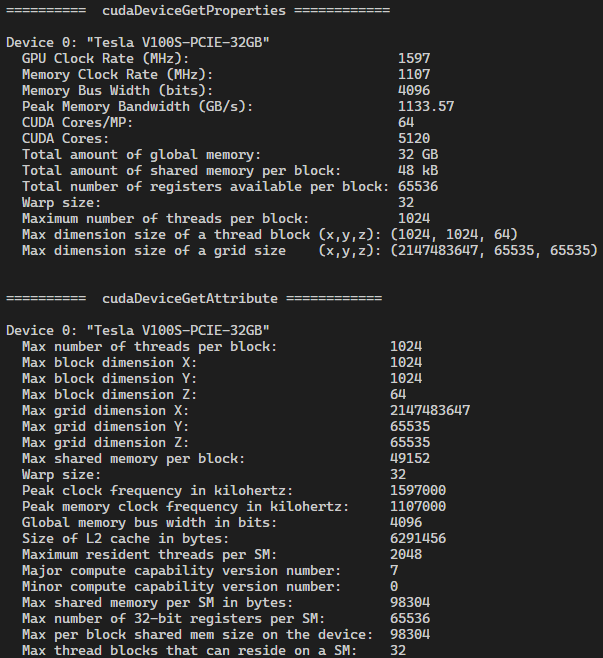
\includegraphics[width=0.8\linewidth]{images/hardware.png}
    \caption{Strojna oprema naprave}
\end{figure}
V tem koraku sem naredil meritve paraleliziranega algoritma, sekvenčnega algoritma ter sekvenčnega algoritma v C-ju (brez CUDA, v gcc compilerju - za testiranje razlike med nvcc ter gcc).\\
Uporabil sem 11 verzij ene slike, katerih resolucija se enakomerno raztega med 10px širine ter 9148px širine (slika je približno kvadratna, tako da je razmerje približno 1:1), vse tri verzije programa pa sem ponovil 20-krat.\\
Za konec sem pa primerjal še sliko \textit{kolesar-neq.jpg} iz predavanj.\\
Merjenje časa poteka od konca branja slike do začetka izdelave nove slike (ta dva ukaza sta input in output, zato dolžina njunega izvajanja ni odvisna od algoritma za histogram ter pretvorbo). Program kot argument sprejme ime slike, ki jo želimo pretvoriti in pa število ponovitev, izračuna pa povprečje vseh ponovitev. Za testiranje vseh treh algoritmov sem naredil bash skripto, ki požene vse tri programe z enako sliko ter enakim številom ponovitev.\\\\
\begin{center}
\begin{tabular}{|m{2.9cm}|m{2cm}|m{2.5cm}|m{2.5cm}|} 
 \hline
 \textbf{Slika} & \textbf{Paralelno [ms]} & \textbf{Sekvenčno (CUDA) [ms]} & \textbf{Sekvenčno (C) [ms]} \\ 
 \hline
 \textbf{\textit{sun00.jpg}, 10px x 10px} & 0.3 & 0.01 & 0.01 \\ 
 \hline
 \textbf{\textit{sun01.jpg}, 922px x 918px} & 0.71 & 19.67 & 17.78 \\ 
 \hline
 \textbf{\textit{sun02.jpg}, 1836px x 1829px} & 1.78 & 63.73 & 56.78 \\ 
 \hline
 \textbf{\textit{sun03.jpg}, 2750px x 2739px} & 3.46 & 137.64 & 123.43 \\ 
 \hline
 \textbf{\textit{sun04.jpg}, 3664px x 3650px} & 7.12 & 242.35 & 215.81 \\ 
 \hline
 \textbf{\textit{sun05.jpg}, 4578px x 4560px} & 10.26 & 378.53 & 336.36 \\ 
 \hline
 \textbf{\textit{sun06.jpg}, 5492px x 5471px} & 14.41 & 537.85 & 483.15 \\ 
 \hline
 \textbf{\textit{sun07.jpg}, 6406px x 6381px} & 19.25 & 718.64 & 643.75 \\ 
 \hline
 \textbf{\textit{sun08.jpg}, 7320px x 7292px} & 24.5 & 932.65 & 833.11 \\ 
 \hline
 \textbf{\textit{sun09.jpg}, 8234px x 8202px} & 30.49 & 1178.19 & 1047.36 \\ 
 \hline
 \textbf{\textit{sun10.jpg}, 9148px x 9112px} & 37.44 & 1454.16 & 1294.96 \\ 
 \hline
 \textbf{\textit{kolesar-neq.jpg}, 1024px x 640px} & 0.62 & 16.42 & 15.38 \\
 \hline
\end{tabular}
\end{center}
\begin{figure}[!h]
    \begin{minipage}{0.48\textwidth}
        \centering
        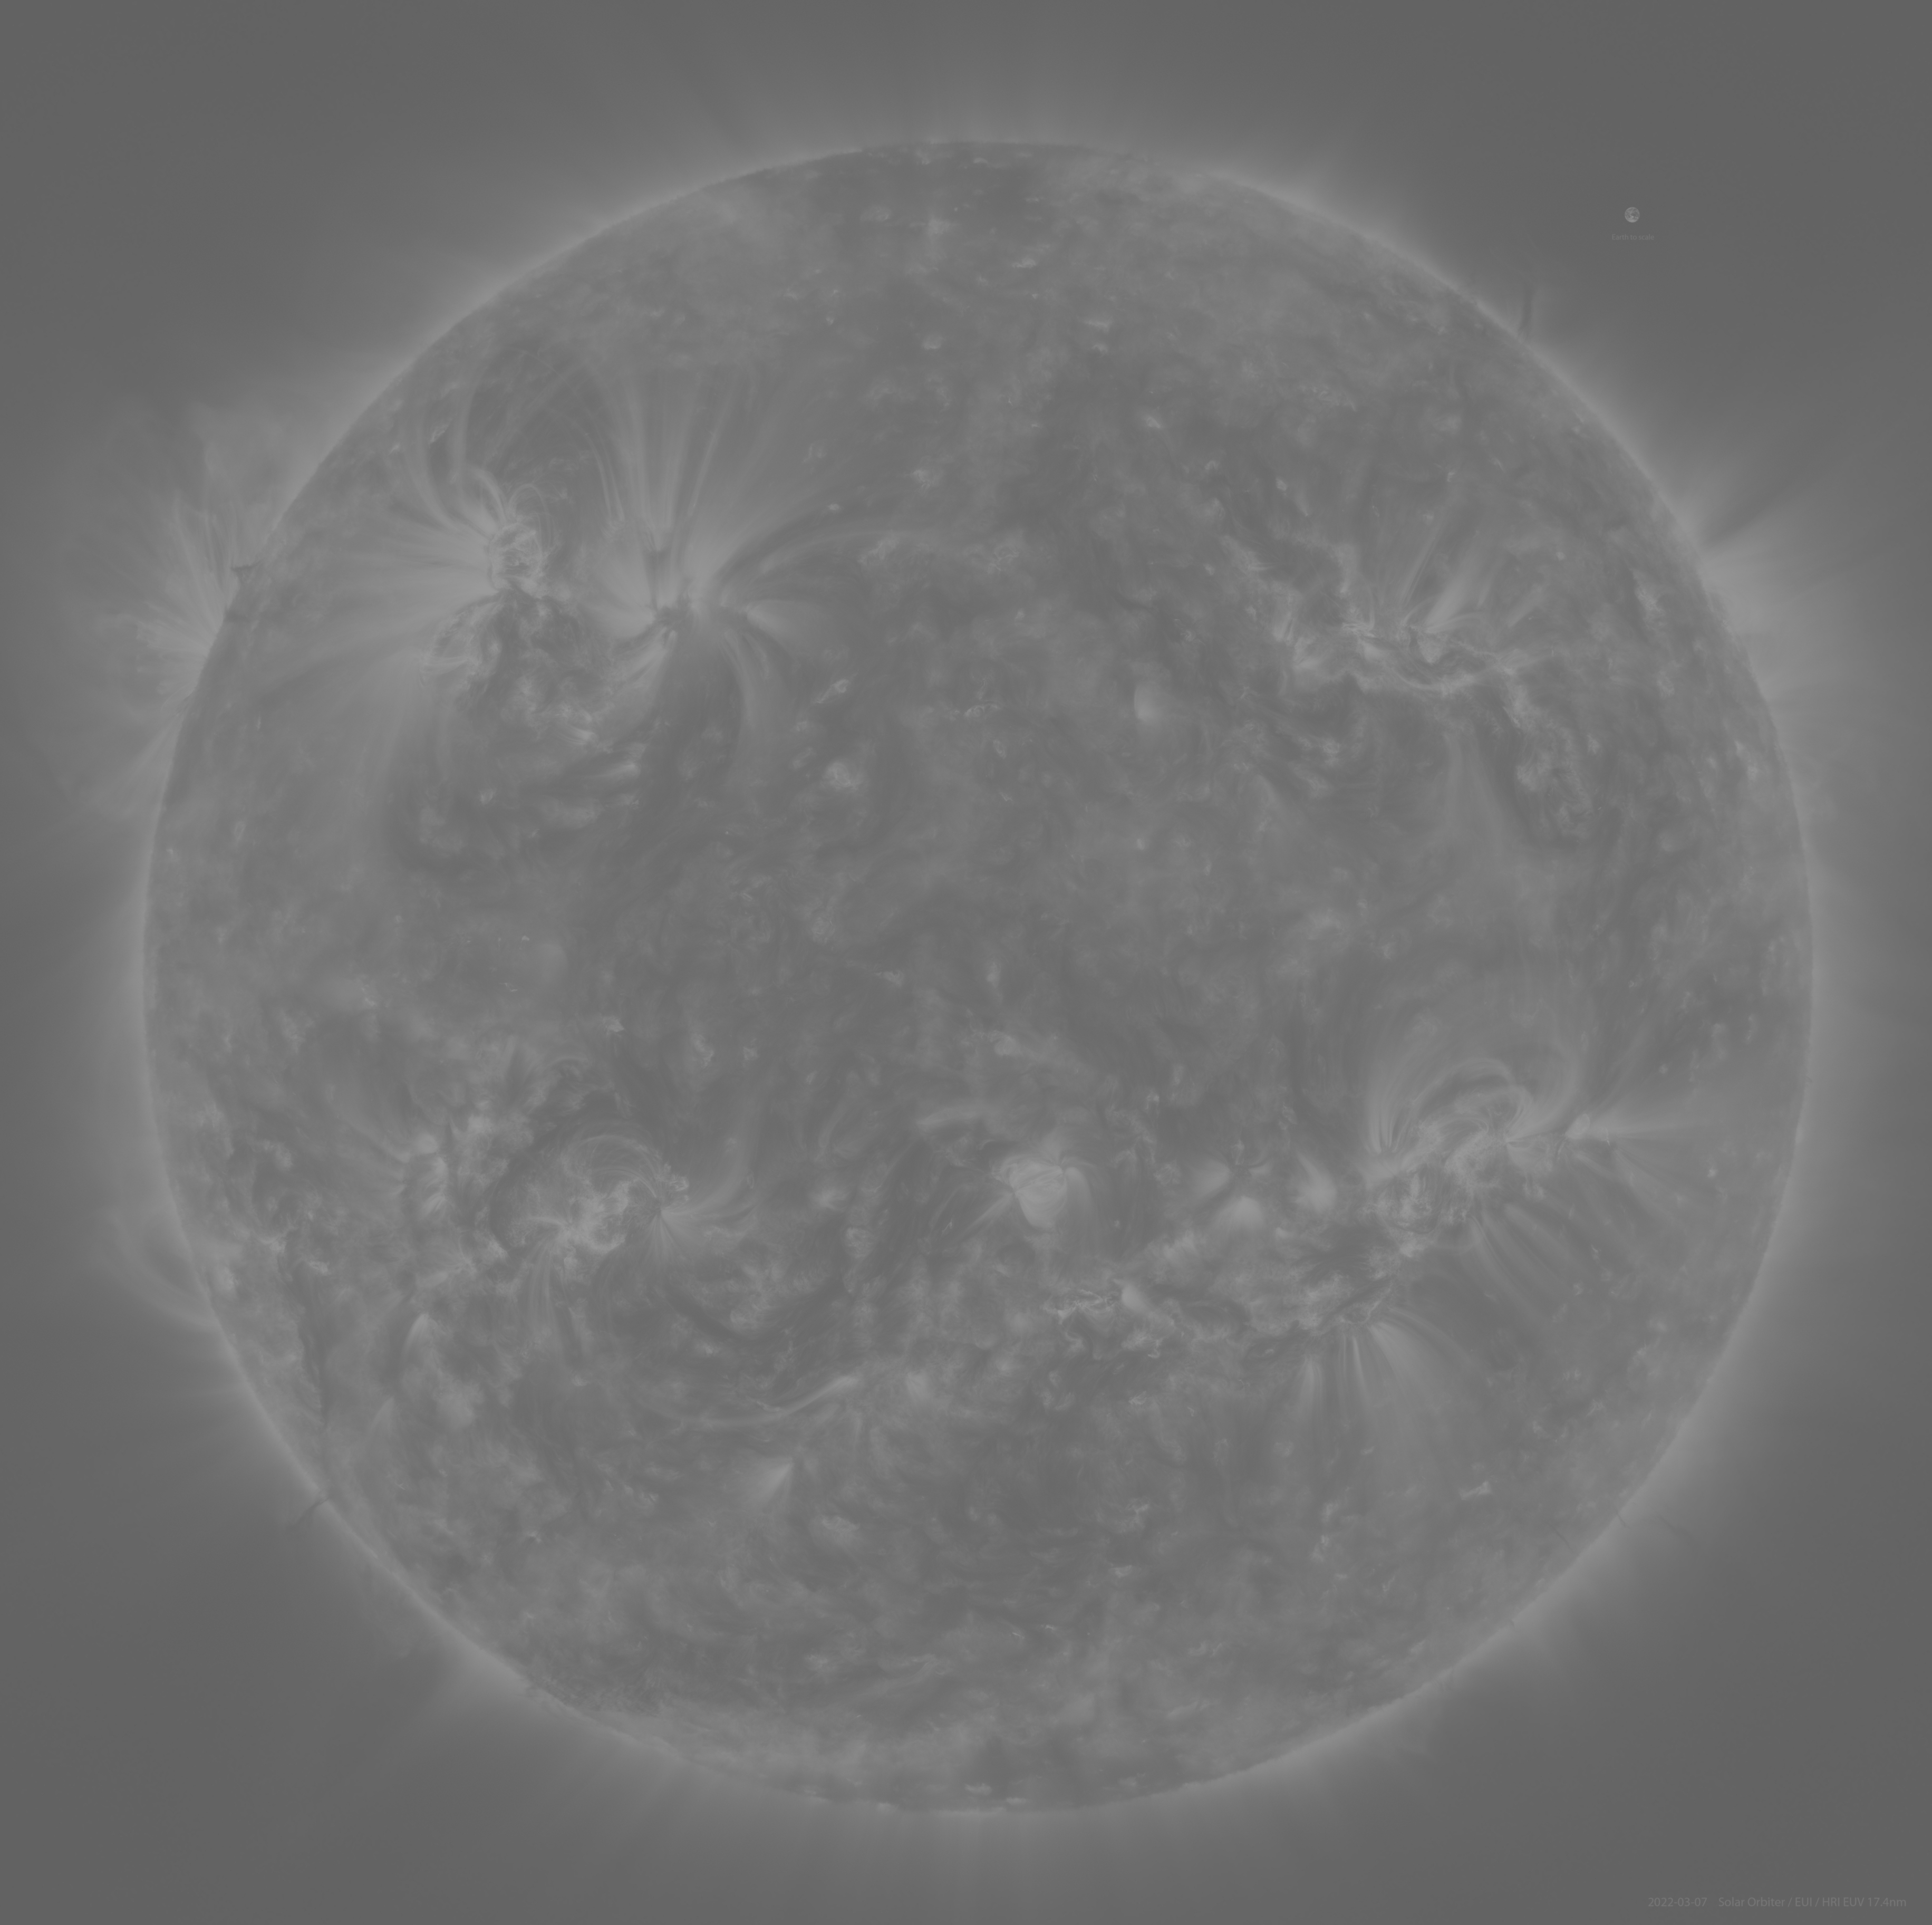
\includegraphics[width=.9\linewidth]{images/sun.jpg}
        \caption{sun.jpg}
    \end{minipage}\hfill
    \begin{minipage}{0.48\textwidth}
        \centering
        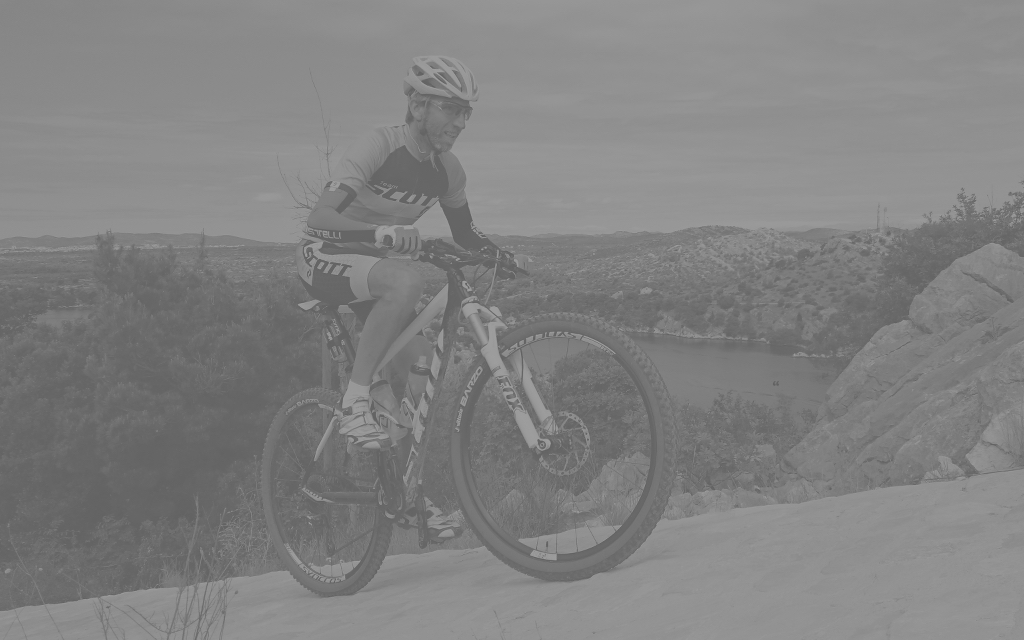
\includegraphics[width=.9\linewidth]{images/kolesar-neq.jpg}
        \caption{kolesar-neq.jpg}
    \end{minipage}
    \caption{Sliki, uporabljeni v eksperimentu}
\end{figure}
\clearpage
\section{Rezultati in diskusija}
\subsection{Primeri enačevanja}
\begin{figure}[!h]
    \begin{minipage}{0.48\textwidth}
        \centering
        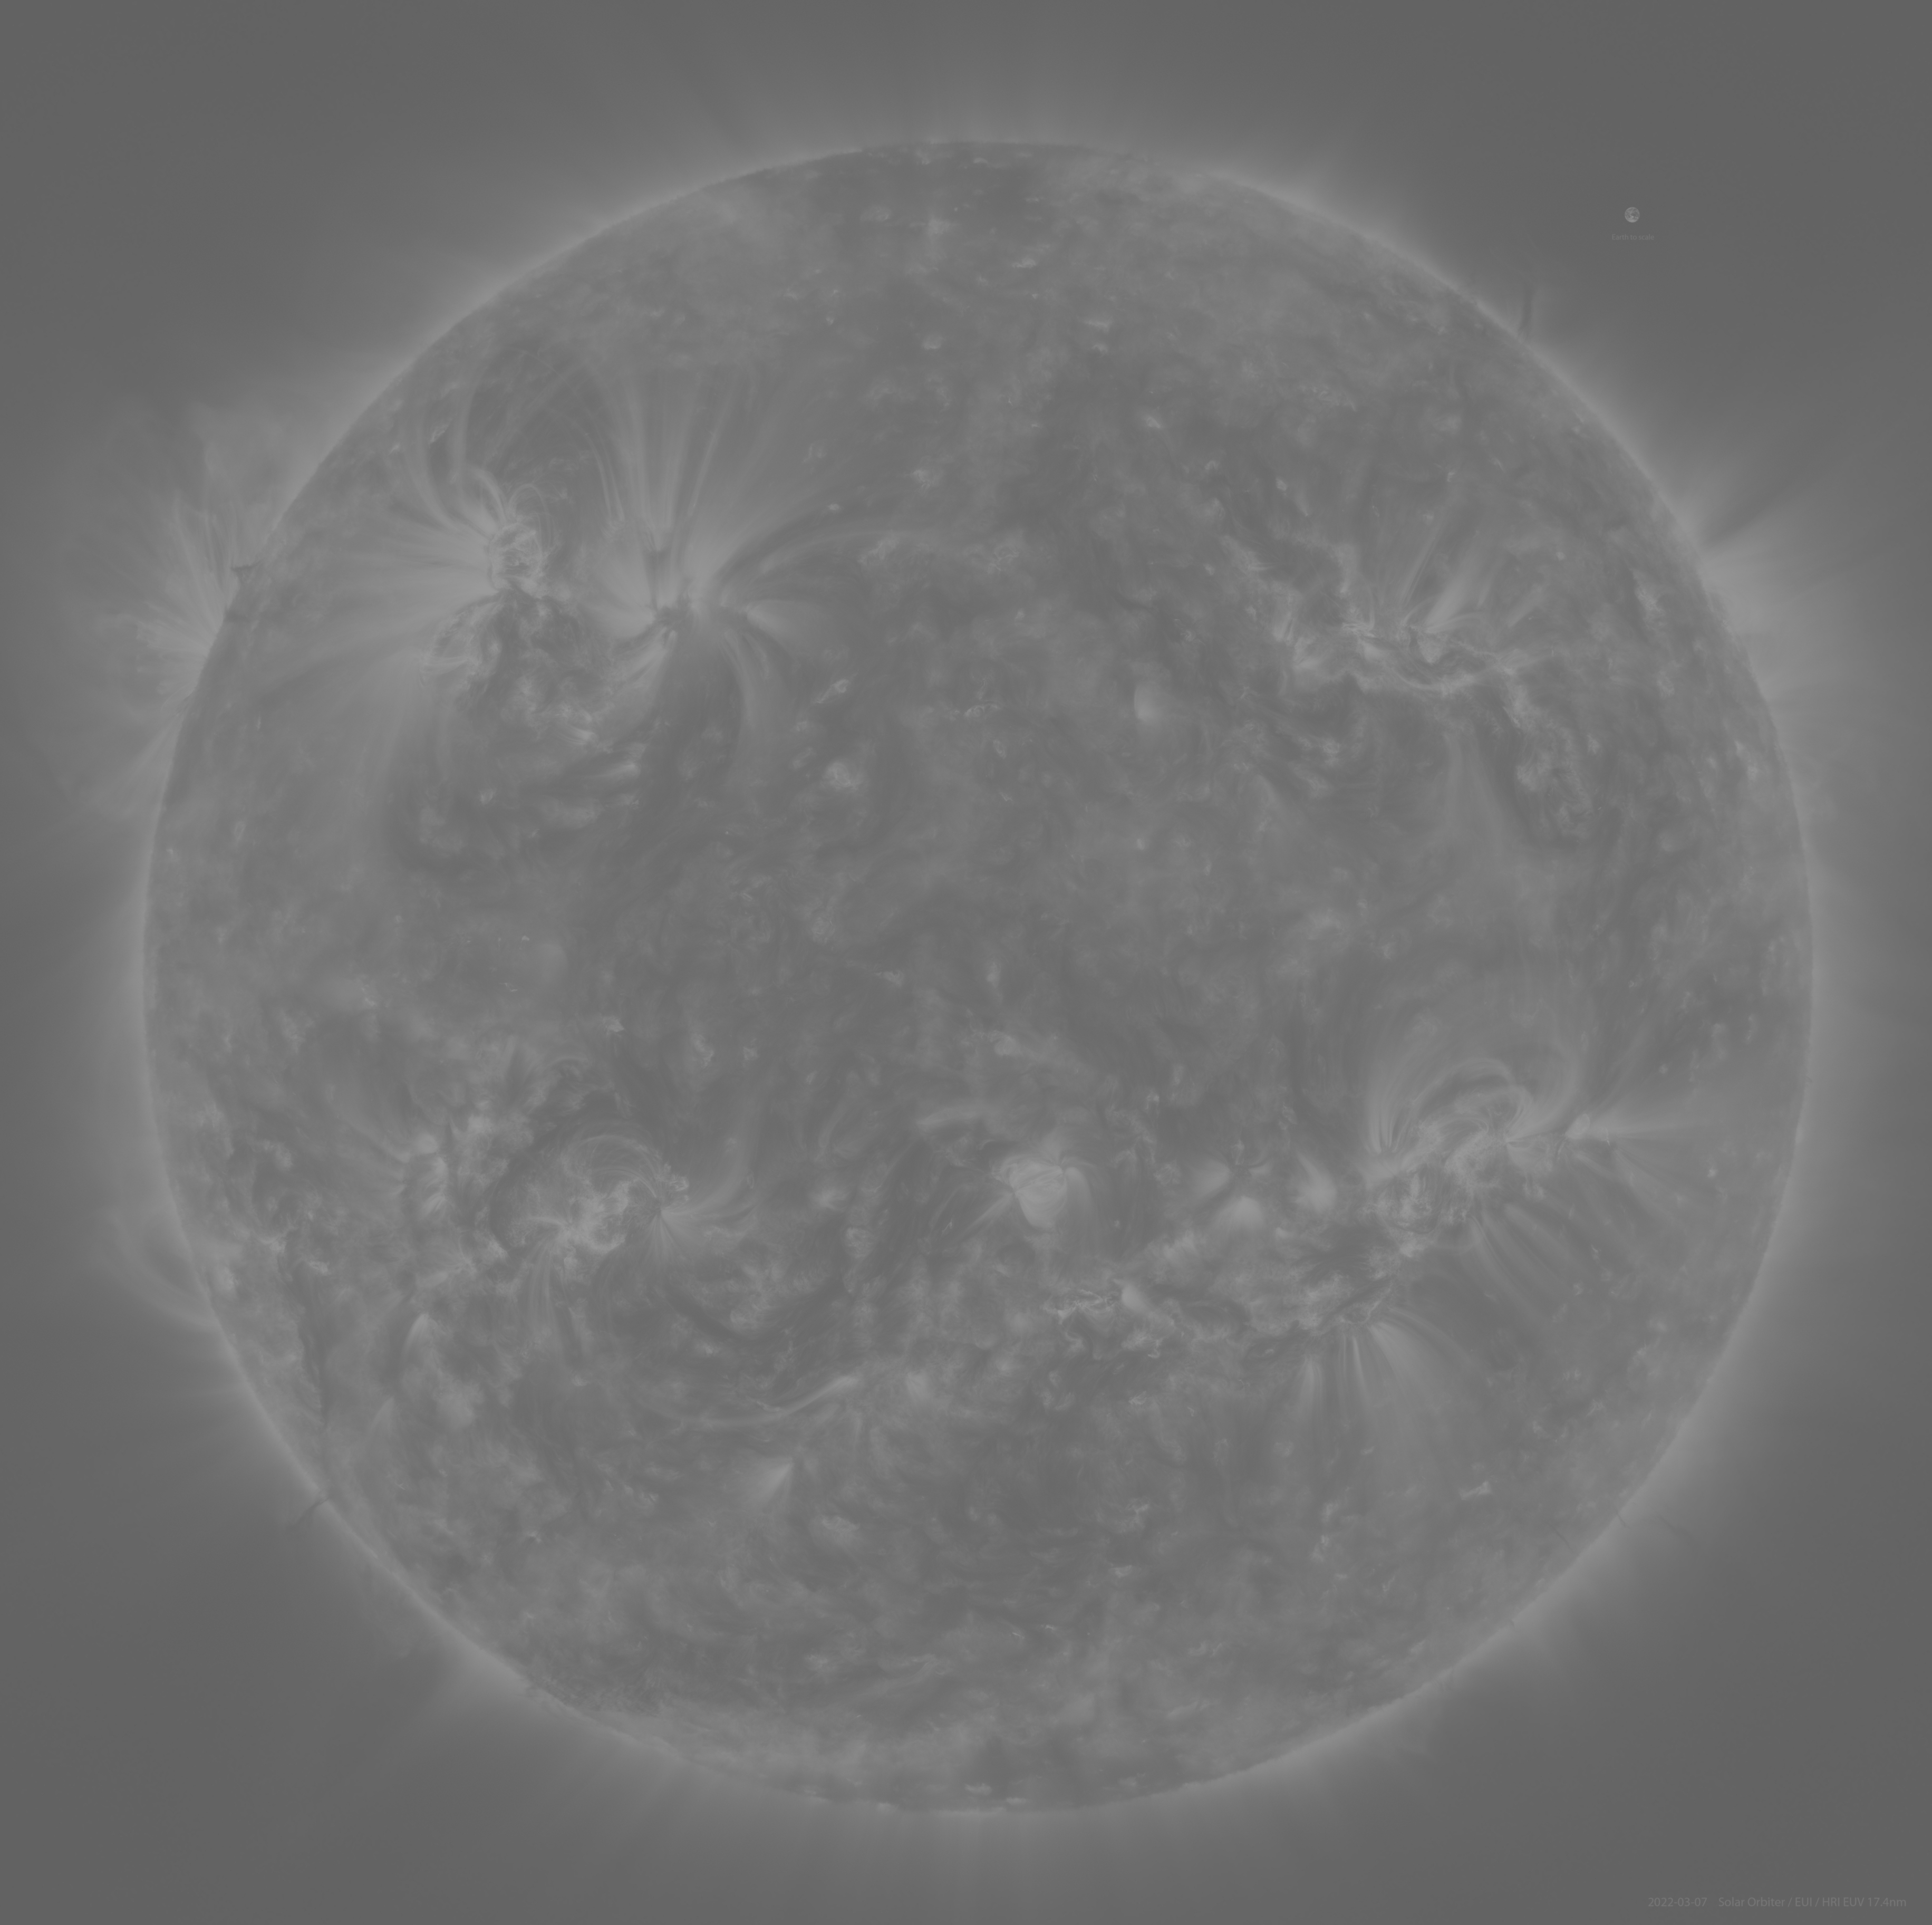
\includegraphics[width=.9\linewidth]{images/sun.jpg}
        \caption{sun.jpg}
    \end{minipage}\hfill
    \begin{minipage}{0.48\textwidth}
        \centering
        \includegraphics[width=.9\linewidth]{images/sun-output.jpg}
        \caption{kolesar-neq.jpg}
    \end{minipage}
    \caption{Primer enačevanja histograma slike \textit{sun.jpg}}
\end{figure}
\begin{figure}[!h]
    \begin{minipage}{0.48\textwidth}
        \centering
        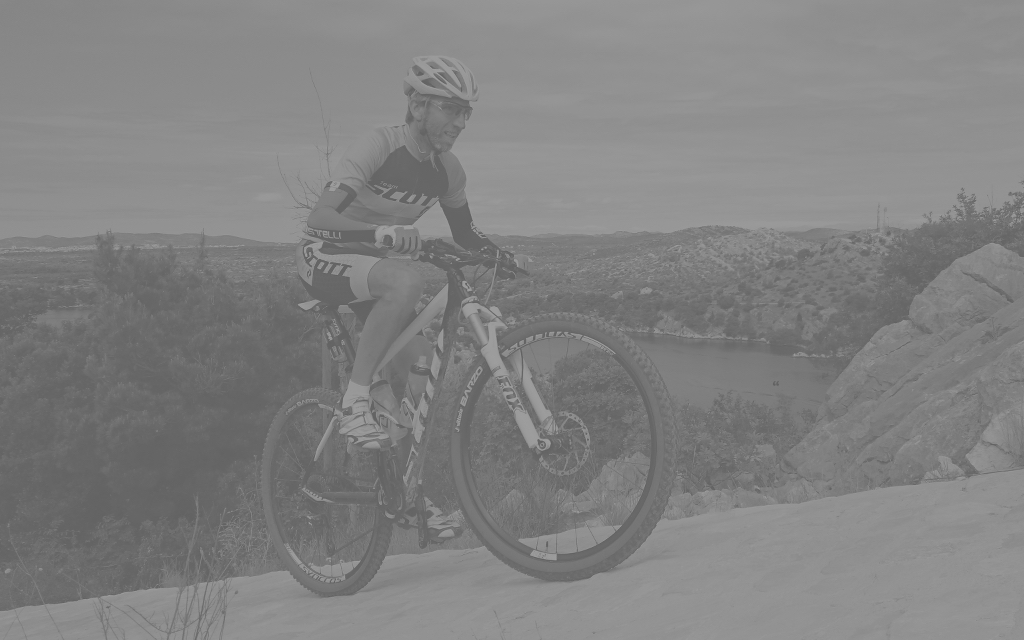
\includegraphics[width=.9\linewidth]{images/kolesar-neq.jpg}
        \caption{sun.jpg}
    \end{minipage}\hfill
    \begin{minipage}{0.48\textwidth}
        \centering
        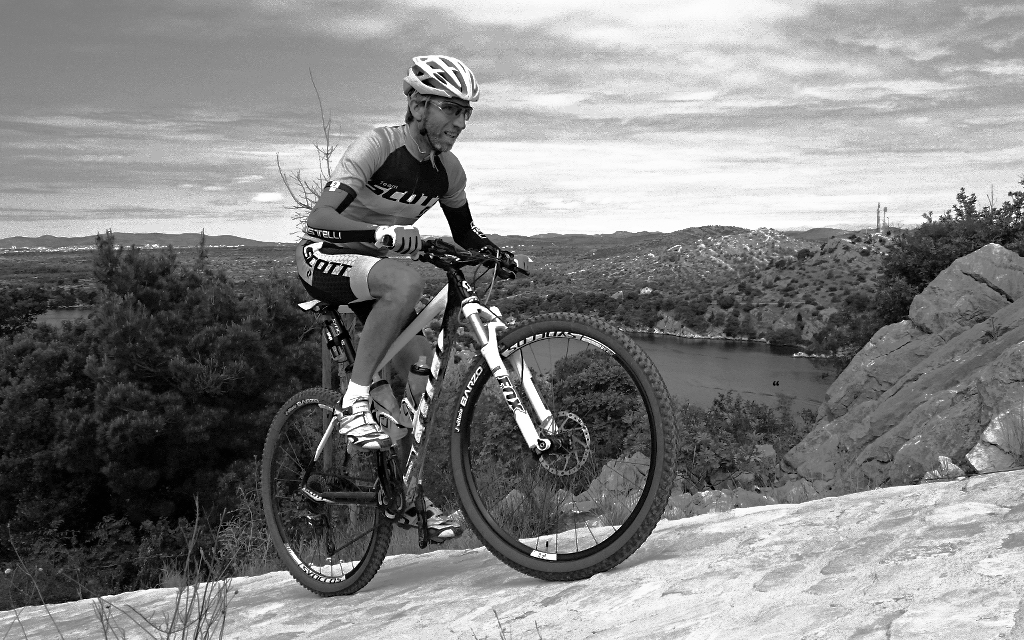
\includegraphics[width=.9\linewidth]{images/kolesar-neq-output.jpg}
        \caption{kolesar-neq.jpg}
    \end{minipage}
    \caption{Primer enačevanja histograma slike \textit{kolesar-neq.jpg}}
\end{figure}
\clearpage
\subsection{Primerjava hitrosti}
Več kot očitno je, da se pri večjih slikah bolj splača uporabiti paralelno verzijo programa. Po velikosti \textit{1836px x 1829px} je pospešitev enakomerna, približno 37x hitrejša. Točni časi so zapisani v tabeli v sekciji eksperiment.
\begin{figure}[!h]
    \centering
    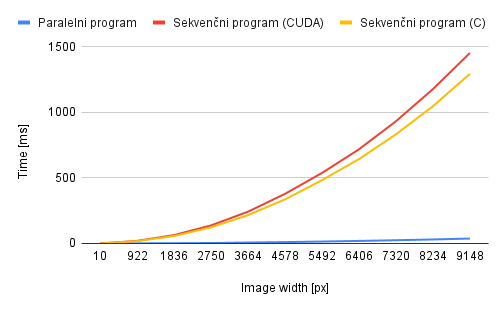
\includegraphics[width=1\linewidth]{images/chart.png}
    \caption{Graf povprečne hitrosti algoritma za 11 različnih velikosti slike \textit{sun.jpg}}
\end{figure}
\clearpage
\subsection{Srečanje hitrosti med paralelnim in sekvenčnim programom}
Prva slika (10px širine) je hitrejša v sekvenčnem algoritmu, zato sem naredil poizkuse do katere velikosti se bolj splača sekvenčna verzija algoritma.\\
Spodnji graf prikazuje, da se hitrosti križata točno pri širini slike 100px. Višina te slike je 99px, torej se algoritma sekata pri 9900 pikslih.\\
Čas pri paralelnem algoritmu je pri majhnih slikah konstanten, ker predvidevam, da se porabi konstantna količina časa za razporejanje niti. To je tudi razlog, zakaj je paralelni algoritem počasnejši pri manjših številih pikslov.
\begin{figure}[!h]
    \centering
    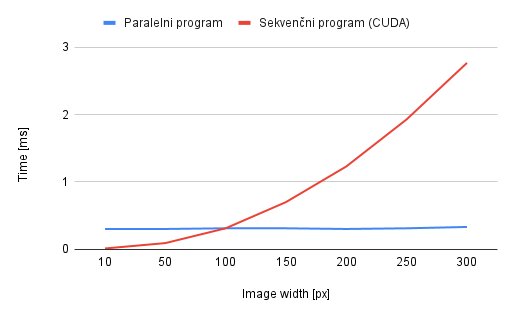
\includegraphics[width=1\linewidth]{images/small-chart.png}
    \caption{Graf povprečne hitrosti algoritma za 11 različnih velikosti slike \textit{small-sun.jpg}}
\end{figure}
\clearpage
\section{Zaključek}
V raziskavi sem ugotovil, da faktor, kolikokrat hitrejši je paralelni algoritem od sekvenčnega, narašča do približno 3358044 pikslov, potem pa postane enakomerna (pibližno 37x hitrejši). Pri 9900 pikslih je meja, do katere se bolj splača uporabljati sekvenčni algoritem, saj razporejanje niti vzame konstantno količino časa.\\
\subsection{GCC}
Kot zanimivost bi poudaril, da sem v mojem testiranju ugotovil tudi, da je sekvenčni program, preveden z \textit{gcc} prevajalnikom konstantno za približno 1.1x hitrejši od programa prevedenega z \textit{nvcc}.
\end{document}
